\section{Tarjan}

\subsection{割点}
\par \noindent 无向连通图中,如果删除某点后(连边删除),图变成不连通,则称该点为【割点】。
\par \noindent 顶点u是【割点】,当且仅当满足下面其一:
\begin{itemize}
\item 特判树根:$u$ 为树根,且 $u$ 有多于一个子树
\item $u$ 不为树根:在递归树上 $u$ 有子结点 $v$,满足: $dfn[u]\leq low[v]$
\end{itemize}

\begin{minted}{c++}
namespace CutPoint {
    int dfn[maxn], low[maxn], timestamp, rt;
    bool cut[maxn];      // 记录点 i 是不是割点
    
    void tarjan(int u, int fa) {
        dfn[u] = low[u] = ++timestamp;
        int child_count = 0;
        for (int i = h[u]; i != -1; i = ne[i]) {
            int v = e[i];
            if (!dfn[v]) {
                tarjan(v, u);
                low[u] = min(low[u], low[v]);
                child_count++;
                if (low[v] >= dfn[u]) {
                    // child_count++;有的放在这里好像也对
                    if (u != rt || child_count > 1) // 根节点特判,v最多走到u走不到u上面去
                        cut[u] = 1;
                }
            } else if(v != fa)
                low[u] = min(low[u], dfn[v]);
        }
    }
}using namespace CutPoint;

int main()
{
    for (int i = 1; i <= n; i++)
        if (!dfn[i])
            rt = i, tarjan(i, 0);
    return 0;
}
\end{minted}

\subsection{桥}
\par \noindent 无向连通图中,如果删除某边后,图变成不连通,则称该边为【割边】。
\begin{minted}{c++}
namespace CutEdge {
    int timestamp, low[maxn], dfn[maxn];
    bool is_bridge[maxm];
    void tarjan(int u, int from) {
        dfn[u] = low[u] = ++timestamp;
        for (int i = h[u]; i != -1; i = ne[i]) {
            int v = e[i];
            if (!dfn[v]) {
                tarjan(v, i);
                low[u] = min(low[u], low[v]);
                if (low[v] > dfn[u]) is_bridge[i] = is_bridge[i^1] = 1;// 该边是桥
            }
            else if (i != (from ^ 1))
                low[u] = min(low[u], dfn[v]);
        }
    }
}
\end{minted}

\subsection{有向图强连通分量 \& 缩点}
\par \noindent 如果有向图中任意两点都有相互可达的路径,则称此图为强连通图。有向图G的极大强连通子图称为G的\textbf{强连通分量(SCC)} 。若两点相互可达,则它们必在同一个环中。

\par \noindent 性质:
\begin{itemize}
\item 强连通分量缩成一点,则形成一个有向无环图DAG。
\item tarjan的过程求出的是反拓扑序
\end{itemize}

\begin{minted}{c++}
// low[u] 从u子树中的结点出发,走一条B边或者C边可以到达的v的dfn最小值,并且要求v还要能够到达u(等价于v在栈里)
namespace SCC {
    int dfn[maxn], low[maxn], c[maxn];    // c[i] 表示节点 i 所属的 scc 编号 
    int scccnt = 0, timestamp;
    bool instack[maxn];
    vector<int> scc[maxn];
    stack<int> s;
    void tarjan(int u) {
        dfn[u] = low[u] = ++timestamp;
        s.push(u), instack[u] = 1;
        for (int i = h[u]; i != -1; i = ne[i]) {
            int v = e[i];
            if (!dfn[v]) // T边 祖先->孩子
                tarjan(v), low[u] = min(low[u], low[v]); //B边 孩子->祖先
            else if (instack[v])
                low[u] = min(low[u], dfn[u]); 
        }
        if (dfn[u] == low[u]) {
            ++scccnt;
            int y;
            do {  //退栈把整个强连通分量都弹出来
                y = s.top(), s.pop();
                c[y] = scccnt, instack[y] = 0;
                scc[scccnt].push_back(y); // 哪些点缩成编号是 scccnt 
                // for(auto x : G[y]) dp[c[y]] = dp[c[x]] 反拓扑序 
            } while (y != u);
        }
    }
    // 缩点
    void shrink() {
        for (int u = 1; u <= n; u++) {
            for (int i = h[u]; i != -1; i = ne[i]) {
                int v = e[i];
                if (c[u] == c[v]) continue; // 处在同一个联通块
                // add_scc_edge(c[x], c[y]);
            }
        }    
    }
}
\end{minted}
\subsection{求无向图点双连通分量 \& 缩点【圆方树】}
\begin{figure}[H]
        \centering
        \par 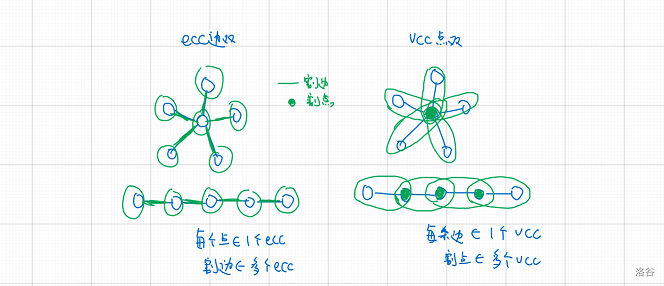
\includegraphics[width=10cm]{images/ecc.png}
\end{figure}
\par \noindent 在一个无向图中,若任意两点间至少存在两条 “点不重复” 的路径,则说这个图是点双连通的,在一个无向图中,点双连通的极大子图称为\textbf{点双连通分量} 。
~\\
\par \noindent 点双连通图定义等价于:任意两条边都在同一个简单环中。
~\\
\par \noindent 【点双联通分量vDCC】:分量中没有割点,每条边属于1个点双,割点属于多个点双。

\begin{minted}{c++}
namespace vDCC {
    int dfn[maxn], low[maxn], timestamp = 0, rt = 0, dcccnt = 0;
    bool cut[maxn];      // 记录点 i 是不是割点
    stack<int> stk;
    vector<int> dcc[maxn];
    void tarjan(int u, int fa) {
        dfn[u] = low[u] = ++timestamp;
        stk.push(u);
        if (u == rt && h[u] == -1) {       // 孤立点,单独成图 
            dcc[++dcccnt].push_back(u);
            return;
        }
        int child_count = 0;
        for (int i = h[u]; i != -1; i = ne[i]) {
            int v = e[i];
            if (!dfn[v]) {
                tarjan(v, u);
                low[u] = min(low[u], low[u]);
                child_count++;
                if (low[v] >= dfn[u]) {    // u是割点或根 
                    if (u != rt || child_count > 1) cut[u] = 1;
                    ++dcccnt;
                    int y;
                    do {
                        y = stk.top(), stk.pop();
                        dcc[dcccnt].push_back(y);
                    } while (y != v);
                    dcc[dcccnt].push_back(u);
                }
            } else if(v != fa)
                low[u] = min(low[u], dfn[v]);
        }
    }
    int solve(int n) {
        for (int i = 1; i <= n; i++)
            if (!dfn[i])
                rt = i, tarjan(i, 0);
        return dcccnt; // 返回点双连通分量个数 v-dcc
    }
    void add_vdcc_edge(int u, int v){}
    
    int num, new_id[maxn], c[maxn];
    void shrink() {
        num = dcccnt;
        // 给割点编号
        for (int i = 1; i <= n; i++)
            if (cut[i])
                new_id[i] = ++num;
        for (int i = 1; i <= dcccnt; i++) {
            for (int j = 0; j < (int)dcc[i].size(); j++) {
                int x = dcc[i][j];
                if (cut[x])
                    add_vdcc_edge(i, new_id[x]), add_vdcc_edge(new_id[x], i);
                else
                    c[x] = i;           // 除了割点之外,标记其它的点只属于一个 v-DCC
            }
        }
    }
}using namespace vDCC;
\end{minted}
\par \noindent 对每个点双,新建一个方点来表示。点双中所有圆点向这个方点连边,原无向图 $\to$ 一棵树
\par \noindent 
\begin{figure}[H]
        \centering
        \par 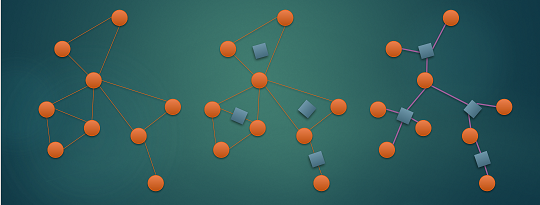
\includegraphics[width=10cm]{images/ecc-tree.png}
\end{figure}

\par \noindent 圆方树的性质:
\begin{enumerate}
\item 圆点方点相间
\item 在圆方树中,原来的每个点对应一个 \textbf{圆点},每一个点双对应一个 \textbf{方点}。
\item 对于每一个度数 $=1$ 的圆点,都对应唯一方点
\item 原图的割点是圆方树中度数 $>1$ 的圆点
\item 原图中每条边,都对应唯一方点 $x$
\item 无论取哪个点为根开始dfs建圆方树,圆方树的形态是一样的
\end{enumerate}
\begin{minted}{c++}
// 小粉图博客 圆方树构建过程
#include <cstdio>
#include <vector>
#include <algorithm>

const int MN = 100005;

int N, M, cnt;
std::vector<int> G[MN], T[MN * 2];

int dfn[MN], low[MN], dfc;
int stk[MN], tp;

void Tarjan(int u) {
    printf("  Enter : #%d\n", u);
    low[u] = dfn[u] = ++dfc; // low 初始化为当前节点 dfn
    stk[++tp] = u; // 加入栈中
    for (int v : G[u]) { // 遍历 u 的相邻节点
        if (!dfn[v]) { // 如果未访问过
            Tarjan(v); // 递归
            low[u] = std::min(low[u], low[v]); // 未访问的和 low 取 min
            if (low[v] == dfn[u]) { // 标志着找到一个以 u 为根的点双连通分量 试了试>= 同样正确
                ++cnt; // 增加方点个数
                printf("  Found a New BCC #%d.\n", cnt - N);
                // 将点双中除了 u 的点退栈,并在圆方树中连边
                for (int x = 0; x != v; --tp) {
                    x = stk[tp];
                    T[cnt].push_back(x);
                    T[x].push_back(cnt);
                    printf("    BCC #%d has vertex #%d\n", cnt - N, x);
                }
                // 注意 u 自身也要连边(但不退栈)
                T[cnt].push_back(u);
                T[u].push_back(cnt);
                printf("    BCC #%d has vertex #%d\n", cnt - N, u);
            }
        } else low[u] = std::min(low[u], dfn[v]); // 已访问的和 dfn 取 min
    }
    printf("  Exit : #%d : low = %d\n", u, low[u]);
    printf("  Stack:\n    ");
    for (int i = 1; i <= tp; ++i) printf("%d, ", stk[i]);
    puts("");
}

int main() {
    scanf("%d%d", &N, &M);
    cnt = N; // 点双 / 方点标号从 N 开始
    for (int i = 1; i <= M; ++i) {
        int u, v;
        scanf("%d%d", &u, &v);
        G[u].push_back(v); // 加双向边
        G[v].push_back(u);
    }
    // 处理非连通图
    for (int u = 1; u <= N; ++u)
        if (!dfn[u]) Tarjan(u), --tp;
        // 注意到退出 Tarjan 时栈中还有一个元素即根,将其退栈
    return 0;
}
\end{minted}

\subsection{求无向图边双连通分量 \& 缩点}
\par \noindent \textbf{边双连通} 如果任意两点至少存在两条边不重复路径,则称该图为边双连通的。
~\\
\par \noindent 【边双联通分量ecc】:分量中没有割边,每个点属于1个边双,割边属于多个边双。

\begin{minted}{c++}
namespace eDCC {
    int dfn[maxn], low[maxn], timestamp, dcnt = 0;
    int c[maxn]; // 缩点后的编号
    bool is_bridge[maxn];
    void tarjan(int u, int from) {
        dfn[u] = low[u] = ++timestamp;
        // stk.push(u);
        for (int i = h[u]; i != -1; i = ne[i]) {
            int v = e[i];
            if (!dfn[v]) {
                tarjan(v, i);
                low[u] = min(low[u], low[v]);
                if (low[v] > dfn[u]) is_bridge[i] = is_bridge[i^1] = 1;// 该边是桥
            }
            else if (i != (from ^ 1))
                low[u] = min(low[u], dfn[v]);
        }
        // 栈的方式缩点
        // if(dfn[u] == low[u]) {
        //     ++dcnt;
        //     int y;
        //     do{
        //         y = stk.top();stk.pop();
        //         c[y] = dcnt;
        //     }while(y != u);
        // }
    }
    // 先找出桥 然后dfs不走桥标记点 看出染色的过程
    void dfs(int u, int co) {
        c[u] = co;
        for (int i = h[u]; i != -1; i = ne[i]) {
            int v = e[i];
            // 节点 y 已被访问或者 (x,y) 是桥 
            if (c[v] || is_bridge[i])
                continue;
            dfs(v, co);
        }
    }
    void solve(int n) {
        for (int i = 1; i <= n; i++)
            if (!dfn[i])
                tarjan(i, 0);
        for (int i = 1; i <= n; i++)
            if (!c[i])
                dfs(i, ++dcnt);
    }

    void add_cut_edge(int u, int v) {}
    void shrink() {
        for (int i = 0; i < idx; i += 2) {     // idx 是前向星的个数
            int v = e[i], u = e[i^1];
            if (c[v] == c[u])
                continue;                   // x, y 同属一个 e-DCC, 无事可做
            add_cut_edge(c[u], c[v]);       // 否则将 x, y 加入新图中
        }
    }    
}using namespace eDCC;
\end{minted}